\externaldocument{../main.tex}

In the previous section I took some shortcuts to give a clearer view of the core components of the
6G architecture while highlighting the idea that the future of mobile communication technologies,
while revolutionary for many different reasons, is just a different spin of the Cloud architecture,
which has been proven to be the future of computation time and time again. It's now time to look under the
rug and explore the problems and some potential solutions that have been proposed.

Since most of the solutions are pretty much interchangeable or work together to solve the same
problems I will first explore the single problems and then move to explaining the various solutions
that have been found, if possible with references to some specific techniques that have been
explored in the literature.

The first problem that needs solving is the model size.

If we consider the network architecture introduced in the last section the network nodes will be
partitioned based on their computational power into the different tiers. If we need to place the
different LLMs based on the need of the various users in the network we now need to take into
consideration two different factors:
\begin{itemize}
	\item The latency: we can put all of the big models (like GPT-4, Stable diffusion, LLaMa,
	      etc...) in the CLOUD, while keeping lighter models like (LLaMa7B) closer to the
	      user. Having such an organization would mean that the end users would need to wait for a time proportional to the quality of the response.

	      Clearly, if the intervention of a model such as GPT-4v is required then the request will subsequently experience very big latency due to how big of a leap inside the architecture the message is going to need to do:
	      \begin{itemize}
		      \item Sending the request from END to CLOUD, passing therefore through many
		            different nodes that, at the moment, do not serve any function other
		            than redirecting the request.
		      \item Waiting for the request to be processed and the inference to be made.
		      \item Sending the response from CLOUD to END.
	      \end{itemize}
	      Since the operation of inference is already costly it's much better to be able to do
	      inference (even on bigger models) as close to the edge of the network as possible, which in turn leads us to the next problem

	\item The space and compute: having to load models in memory or even saving them is
	      extremely expensive, that is because of the amount of resources required.
	      As can be seen in \cite{hug-optimization} the dimensions of required VRAM in GPU for LLMs at
	      different ranges of performance (from GPT-3 to bigcoder/starcoder) require between 350 and
	      30 GB of VRAM, which is already extreme for any computing device that might inhabit the Fog, even at the lowest end of the model spectrum.

	      Even the requirements in terms of basic storage are completely out of the capabilities of
	      the majority of devices inside the Fog (175 GB for GPT-3 is a lot, especially if we consider
	      that the user might not have stored locally just the one LLM but might need to deploy different ones for different pourposes).

	      Last but not least, doing inference on the model or training the model will most likely
	      require more compute power than the one available to most of the devices in the Fog.
\end{itemize}

It's clear enough that what is required here is to be able to employ smartly all of the resources at
our disposal to allow efficient training, re-training and fine-tuning operations, while, at the same
time, being able to save more than one model on board in order to serve END devices as fast as possible when necessary. To make matters worse, when fine-tuning a model with users' data the procedure should be done as
securely as possible, meaning that user's data should never leave their device.
The safety hazard should be taken with the utmost caution since we are talking about an
unprecedented amount of data that comes from different spheres of a users' life and in general all
very private e.g. biometric, private audio and video and very precise location information.

\bigskip
\noindent
FEDERATED LEARNING:

Federated Learning is the first distributed learning technique for machine learning models with a
very strong focus on users' data privacy. Google developers came up with the technique to solve the
problem of base model update without access to private data for the word predictor implemented in
Android.

At a very high level FL works by downloading a basic version of the model locally on the device, if
we consider the example of the word predictor the basic information will be the most basic form of
the predictor and dictionary, and then for a certain amount of time or epochs the model will undergo
updates based on local data, in our case we will be talking about updates to the dictionary and new
inference rules; lastly, once the epochs counter is depleated, the resulting model undergoes
gradient backpropagation and the result is encrypted so that private (and reconstructible) data
cannot be inferred by malicious third parties.

Even without a deeper dive in the inner workings of FL it's really easy to see how difficult it is
to extend the above technique to the world of LLMs, having small extremal terminals handling their
own copy of the base model is not possible for two reasons:
\begin{itemize}
	\item \textbf{size}: The models are simply too large to be saved entirely on modern day
		mobile hardware, the only possible solutions to this issue would be to do model
		compression (changing the precision of the float values in the weights matrices of
		the model) or one of the variants of LoRA.

		Furthermore the model would need to be moved repeatedly between the center node and
		the various END nodes participating in the training procedure, that would put
		extreme amounts of strain on the network, even in the case of compression.
	\item \textbf{updating the models}: The fundamental concept of FL is to have a
		decentralized training process thanks to the participation of different nodes in 
		the network, but small nodes such as the END nodes cannot possibly handle LLM
		inference (let us be reminded that all of the current LLM-based applications run in
		cloud and are therefore just frontends that are not running the model locally, like
		the latest Gemini model released by Samsung for 2024). 
\end{itemize}
That said I think that using LoRA, which will be discussed further in the article, alongside FL
makes for an amazing weapon for training of bigger models at the center of the network, being able
to have a series of supercomputers training a new base model that will be later passed on to the
lighter nodes inside the network makes the training procedure much more efficient than it would be
if the training was being handled by just one of the central nodes in the network.

\bigskip
\noindent
SPLIT LEARNING:

Split learning (SL), in a way, is an upgrade of the FL technique.
SL allows model the division of the model in various sub-models that can be trained separately, the
backpropagated gradients can then be sent through the network to the "sibling nodes" to allow them
to procede with their own training as is shown in Figure \ref{img:split-learning}.
The way the model will be divided is dependent on many factors e.g. size of the
model, privacy concerns of the user, level of customization required by the user, network topology
and level of mobility of the user, etc...
Since the variables are many it might be a very good idea to allow the CONTROLLER to handle the
decision on how to split the model. Based on all the different variables it could be possible to
deploy an RLM in the CONTROLLER that is able to chose how to slice the model in order to strike a
balance between having too many different slices, energy efficiency and latency.

SL will be a very powerful tool and a central part of the software architecture deployed alongside
6G since it allows users to have powerful models at their disposal without sending their data to the
cloud (the fine-tuning is done on-device) and without having to wait too long for the training process to be over.
\begin{figure}
	\center
	\phantomcaption
	\label{img:split-learning}
	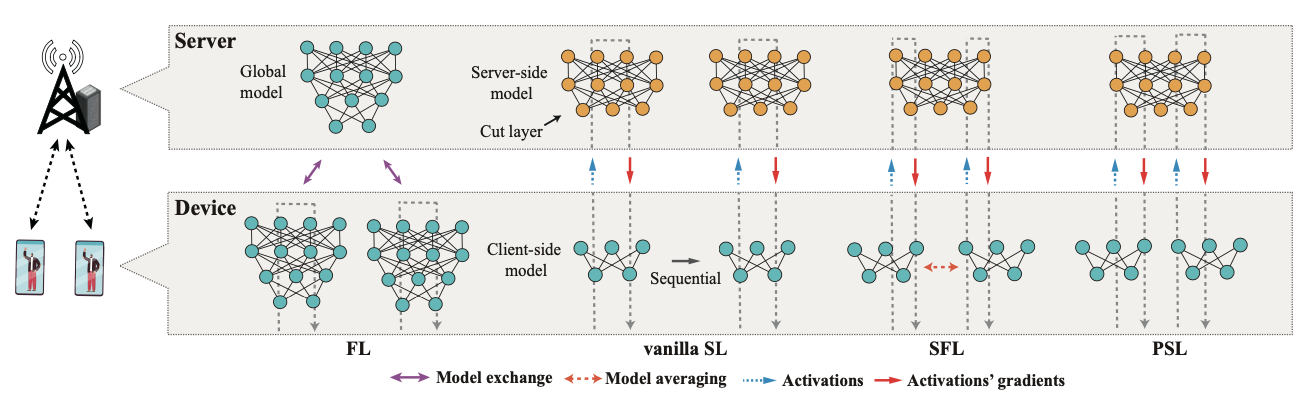
\includegraphics[scale=0.65]{figures/split-learning.png}
	\caption{An example of the structure of a network implementing SL for model trainig
		\cite{split-learning}}
\end{figure}
SL is just a piece of the intricate puzzle that we need to build, it allows us to have fast training
procedures, supposing the model has been divided effectively, but it forces us to have the model
fragmented in different parts of the network and this complicates things because we want the model
to be "local" to the user, or at least the part that has been fine-tuned for his use.
To grant this locality property we will need to have load balancing algorithms or RLMs that can
handle the choice of model migration.

Although SL makes the training process possible while keeping user's private data safe, it
introduces complications on the inference side, depending on the number of sections that the model
has been partitioned into the inference process is going to require the participation of all the
computing elements that store a part of the whole model. This implies a discrete volume of data that
needs to be moved between the various compute elements in order to allow the calculation of the
results.

Since the process leads to a very clear network strain we will be seeing in the following a series
of compression techniques that allow the reduction of the amount of data that need to be moved in
the network to complete the inference process.

\bigskip
\noindent
LOW-RANK ADAPTATION

LOw-Rank Adaptation (LoRA) is a compression technique that freezes the pretrained model weights and injects
trainable rank decomposition matrices into each layer of the Transformer architecture, greatly
reducing the number of training parameters for downstream tasks.

This technique really strikes the point because it's of the utmost importance to be able to reduce
the number of trainable parameters for the constrained devices that will need to face some sort of
fine-tuning procedure in the END layer. Instead of doing a fine-tuning of the complete model we do
the fine tuning of a reduced version of the original weight matrices, the procedure is well
explained by Figure \ref{fig:lora}.
\begin{wrapfigure}{L}{0.5\textwidth}
	\phantomcaption
	\label{fig:lora}
	\centering
	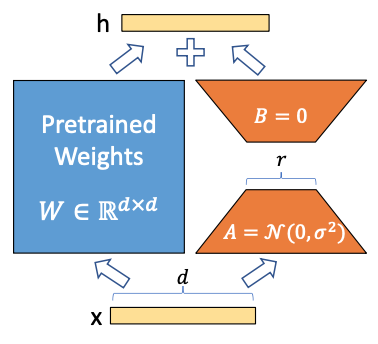
\includegraphics[scale=0.7]{figures/lora.png}
	\caption{The LoRA approach proposed in \cite{lora}}
\end{wrapfigure}
Per the studies made in article \cite{lora}, given a weight matrix $W_0 \in \R^{d \times k}$ we can
actually represent it via a low-rank decomposition like:
\begin{equation}
	W_0 + \Delta W = W_0 + B \cdot A
\end{equation}
where $B \in \R^{d \times r}, A \in \R^{r \times k}$ and the rank $r$ is much smaller than either
$d$ (which is the full rank of the dense layers' decomposition matrices, in the case of GPT-3 the
count can get up to 12.288) or $k$, and these are the ones shown in \ref{fig:lora}. The result is an extremely underdimensioned matrix with respect to the ones that we would have had to work with in origin.

The gradient updates for the matrix $W_0$ are frozen while $A$ and $B$ contain the trainable
parameters.

When utilizing this technique in the field of Transformers (which is the fundamental constituend of
LLM architectures) the empirical results when using GPT-3 175B were the following:
\begin{itemize}
	\item slicing VRAM of up to $2/3$ since there is no need to store Adam optimizer states for
	      the frozen parameters (they went from 1.2 TB to 350GB of VRAM usage).
	\item If the rank of the decomposition was 4 and, of all the transformer matrices, only the
	      value projection and query matrices were adapted the checkpoint size is reduced of
	      circa 10000 times which in turns means very easy model switching due to the
	      forgettable size of LoRA weights.
\end{itemize}
To provide another reason for LoRA, it's really easy to implement next to other techniques. I would
go as far as to say that it's essential to allow the correct implementation of distributed
learning techniques like SL, because even the partial retrain of a network for fine-tuning might be
too expensive for the underpowered nodes at the END of the 6G network. What is even more impressive
is that, by using LoRA, it's possible to change the specialization of the LLM by swapping the A and
B matrices shown in Figure \ref{fig:lora}; this concepts fits perfectly in the frame of having a
split model, if we consider that the part related to the user's specific data (the A and B matrices)
will be living on the END device, we can imagine having a series of different trained low-rank
adapters that can be swapped to change the behaviour of the LLM and make it more adapt to the
situation. If we factor in the fact that having a snapshot of the LoRAs takes (in the case of GPT-3)
35MB because it's only necessary to save the matrices themselves and not all of the weight matrices,
it's very easy to see how doable a development like this would be.

As an additional point of interest, that will not be covered, there have been developments in the
field of LLM optimization and QLoRA was born out of the mix between quantization techniques and
LoRA. The necessity of expanding the LoRA approach was born from the fact that the fine-tuning
operation for a model like LLaMA 65B (full 16 bit fine-tuning) over 780GB of GPU memory are required
and quantization only works at inference time. The approach shown in \cite{qlora} explains how it is
possible to quantize a pre-trained model to 4 bit precision and then backpropagate the gradients
after doing the adapter injection to train them; this revelation renders the memory requirements for
fine-tuning worth considering (less than 48GB of GPU memory).
